% !TEX program = xelatex
% Compile with XeLaTeX
\documentclass[10pt,aspectratio=43]{beamer}
\usepackage{ctex}
\setCJKmainfont{SimSun}
\setCJKsansfont{SimHei}
\setCJKmonofont{KaiTi}

\usetheme{metropolis}
\usecolortheme{default}
\setbeamercolor{frametitle}{bg=blue!70!black,fg=white}
\setbeamerfont{frametitle}{size=\Large,series=\bfseries}
\setbeamercolor{title}{fg=white}
\setbeamercolor{normal text}{fg=darkgray}
\setbeamercolor{item}{fg=orange}

\usepackage{amsmath,amssymb}
\usepackage[table]{xcolor}
\usepackage{booktabs}
\usepackage{array}
\usepackage{graphicx}

\graphicspath{{RTAD/}{PROBLEM1/}{PROBLEM3/}{PROBLEM2/}{BEAMSIZE/}{OVERLAY/}{./}}

\newcommand{\blue}[1]{\textcolor{blue!70!black}{#1}}
\newcommand{\orange}[1]{\textcolor{orange}{#1}}

\title{矩形平顶 DOE 光束整形\\—— 从设计到容差评估}
\author{基于 Romero-Dickey 点对点法 + RTAD 目标 + WGS 优化}
\date{2026 年 5 月}

\begin{document}

% ===================================================================
\begin{frame}[plain]
  \vspace{1.8cm}
  \begin{center}
    \usebeamerfont{title}\inserttitle\\
    \vspace{0.4cm}
    \insertauthor\\
    \vspace{0.3cm}
    \insertdate
  \end{center}
\end{frame}

% ===================================================================
\section{项目目标}

\begin{frame}{项目目标}
  \begin{columns}
    \column{0.55\textwidth}
    设计一片衍射光学元件（DOE），将 532nm 高斯激光束整形成焦平面上的 \orange{矩形平顶光斑}（330\,$\times$\,120\,$\mu$m）。\vspace{0.2cm}

    \begin{table}
      \rowcolors{2}{gray!10}{white}
      \begin{tabular}{p{2.8cm}l}
        \toprule
        \textbf{参数} & \textbf{值} \\
        \midrule
        波长 $\lambda$ & 532\,nm \\
        入射光斑 & 5\,mm ($1/e^2$) \\
        透镜焦距 $f$ & 429\,mm \\
        通光孔径 & 15\,mm \\
        目标光斑 & 330$\times$120\,$\mu$m \\
        网格 $N$ & 2048$\times$2048 \\
        $\beta_x$ / $\beta_y$ & 9.06 / 3.30 \\
        \bottomrule
      \end{tabular}
    \end{table}

    \column{0.45\textwidth}
    \begin{center}
      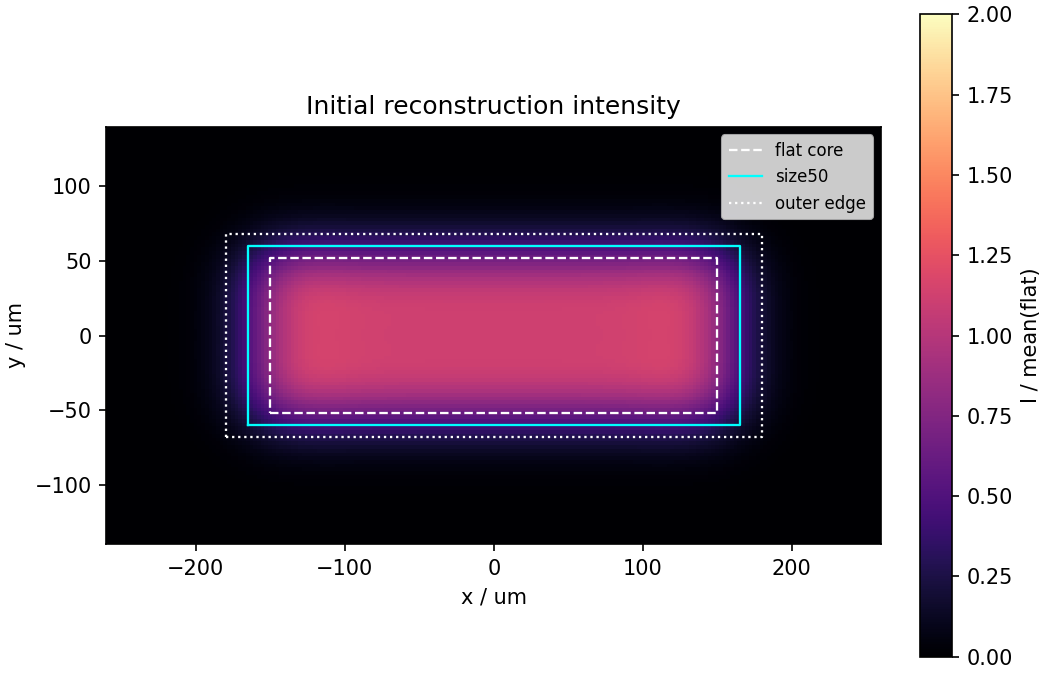
\includegraphics[width=\textwidth]{initial_reconstruction_intensity.png}\\
      {\footnotesize 初始相位 (Phase0) 焦斑}
    \end{center}
  \end{columns}
\end{frame}

% ===================================================================
\section{物理基础}

\begin{frame}{物理基础 \ \ Romero-Dickey 点对点法}
  {\scriptsize Romero \& Dickey, ``Lossless laser beam shaping,'' \textit{J. Opt. Soc. Am. A}, 13(4), 751--760 (1996).}

  \vspace{0.05cm}
  \begin{itemize}
    \item 菲涅尔近似下，用稳相法 (stationary phase) 解析求解高斯$\to$平顶的 DOE 相位
    \item 解的质量由无量纲参数 $\beta$ 决定：
  \end{itemize}
  \[
    \boxed{\;\beta = \frac{2\pi \cdot r_i \cdot R_o}{\lambda \cdot f}\;}
  \]
  \begin{itemize}
    \item $\beta$ 越大 $\to$ 几何光学近似越精确；$\beta<6/\pi\approx 1.91$ 时无合理解
  \end{itemize}

  \vspace{-0.1cm}
  \begin{table}
    \rowcolors{2}{gray!10}{white}
    \footnotesize
    \begin{tabular}{llll}
      \toprule
      \textbf{参数} & \textbf{符号} & \textbf{值} & \textbf{说明} \\
      \midrule
      输入 1/$e$ 幅度半径 & $r_i$ & 1.768\,mm & $=(\text{5mm}/2)/\sqrt{2}$ \\
      x 方向输出尺度 & $R_{ox}$ & 186.2\,$\mu$m & 330\,$\mu$m\,$/\,\sqrt{\pi}$ \\
      y 方向输出尺度 & $R_{oy}$ & 67.7\,$\mu$m & 120\,$\mu$m\,$/\,\sqrt{\pi}$ \\
      x 方向 $\beta$ & $\beta_x$ & 9.06 & 正常 \\
      y 方向 $\beta$ & $\beta_y$ & 3.30 & \orange{限制方向} \\
      \bottomrule
    \end{tabular}
  \end{table}
\end{frame}

% ===================================================================
\begin{frame}{物理基础 \ \ Romero-Dickey 相位公式与初始相位}
  \begin{columns}
    \column{0.5\textwidth}
    \textbf{一维无纲量相位} ($\xi = x/r_i$):
    \[
      \phi(\xi) = \beta \Bigl[
        \tfrac{\sqrt{\pi}}{2}\xi\,\mathrm{erf}(\xi)
        + \tfrac{1}{2}e^{-\xi^{2}}
        - \tfrac{1}{2}
      \Bigr]
    \]
    \textbf{二维可分离}:
    $\phi(x,y) = \beta_x f(x/r_i) + \beta_y f(y/r_i)$

    \column{0.5\textwidth}
    \begin{center}
      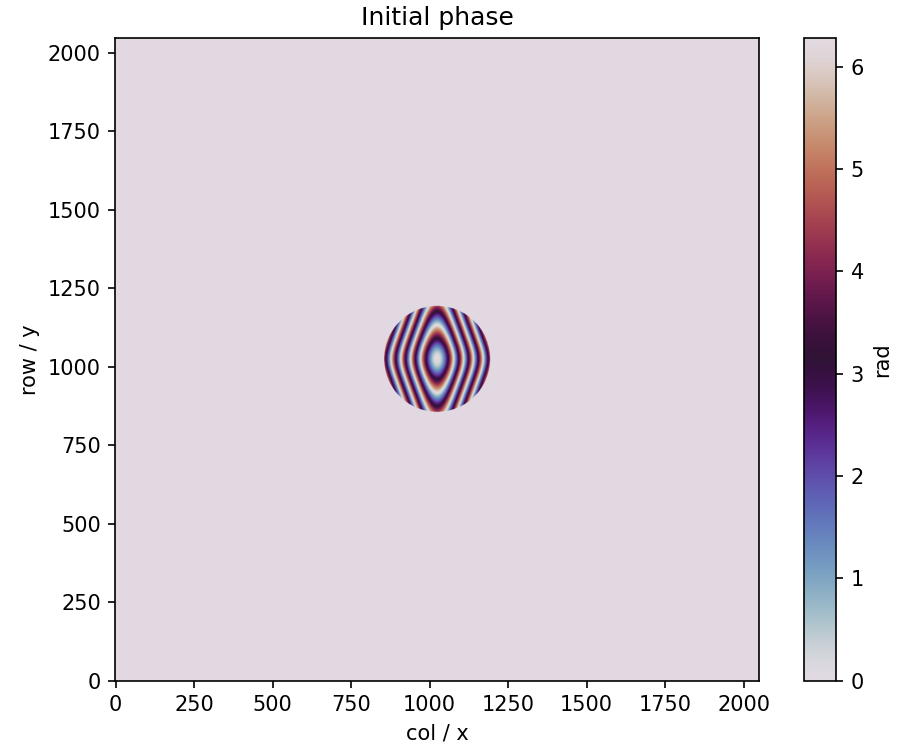
\includegraphics[width=0.82\textwidth]{phase0.png}\\
      {\footnotesize Romero-Dickey 初始相位 phase0 (wrapped $[0,2\pi)$)}
    \end{center}
  \end{columns}

  \vspace{0.15cm}
  \begin{itemize}
    \item 该相位为 \orange{解析解}，无需迭代，直接给出接近目标能量分布的初始相位
  \end{itemize}
\end{frame}

% ===================================================================
\begin{frame}{物理基础 \ \ RTAD 目标函数}
  {\footnotesize Chen et al., ``\ldots high uniformity flat-top beams by RTAD,'' \textit{Opt. \& Laser Tech.}, 186, 112776 (2025).}

  \vspace{0.1cm}
  \textbf{问题}: 传统陡峭边缘目标 $\to$ FFT 频谱泄露 $\to$ 散斑噪声

  \textbf{方案}: 引入 \orange{升余弦 (raised-cosine) 下降边缘}

  \vspace{0.1cm}
  \textbf{升余弦边缘函数}:
  \[
    C(u) = \begin{cases}
      1 & (u \leq u_0) \\[4pt]
      \frac{1}{2}\!\left[1 + \cos\!\left(\pi\frac{u-u_0}{u_1-u_0}\right)\right] & (u_0 < u < u_1) \\[8pt]
      0 & (u \geq u_1)
    \end{cases}
  \]

  \[
    I_{\mathrm{full}}(x,y) = C(|x|; a_0,a_1) \cdot C(|y|; b_0,b_1),\qquad
    A_{\mathrm{full}} = \sqrt{I_{\mathrm{full}}}
  \]
  \begin{itemize}
    \item $a_0 = a_{50}-\Delta x,\; a_1 = a_{50}+\Delta x$（默认 $\Delta x=15\mu$m, $\Delta y=8\mu$m）
    \item 文献: 仿真均匀性 98.8\%, 实验 91.0\%
  \end{itemize}
\end{frame}

% ===================================================================
\begin{frame}{物理基础 \ \ RTAD 目标与截断约束}
  \begin{columns}
    \column{0.55\textwidth}
    \orange{截断 RTAD} — 只约束 $I\geq e^{-2}\approx 13.5\%$ 的信号区

    \begin{table}
      \rowcolors{2}{gray!10}{white}
      \footnotesize
      \begin{tabular}{p{1.7cm}p{3.2cm}}
        \toprule
        \textbf{区域} & \textbf{投影方式} \\
        \midrule
        mask\_flat (纯平顶) & WGS 权重反馈 \\
        mask\_signal (信号区) & 目标振幅约束 \\
        mask\_free (自由区) & MRAF\,$m\cdot E$ \\
        mask\_bg (远背景) & 不约束 ($b\to 1.0$) \\
        \bottomrule
      \end{tabular}
    \end{table}
    \begin{itemize}
      \item 低强度尾迹$\to$自由区，保留物理旁瓣
      \item RMS 均匀性仅在 mask\_flat 计算
    \end{itemize}

    \column{0.45\textwidth}
    \begin{center}
      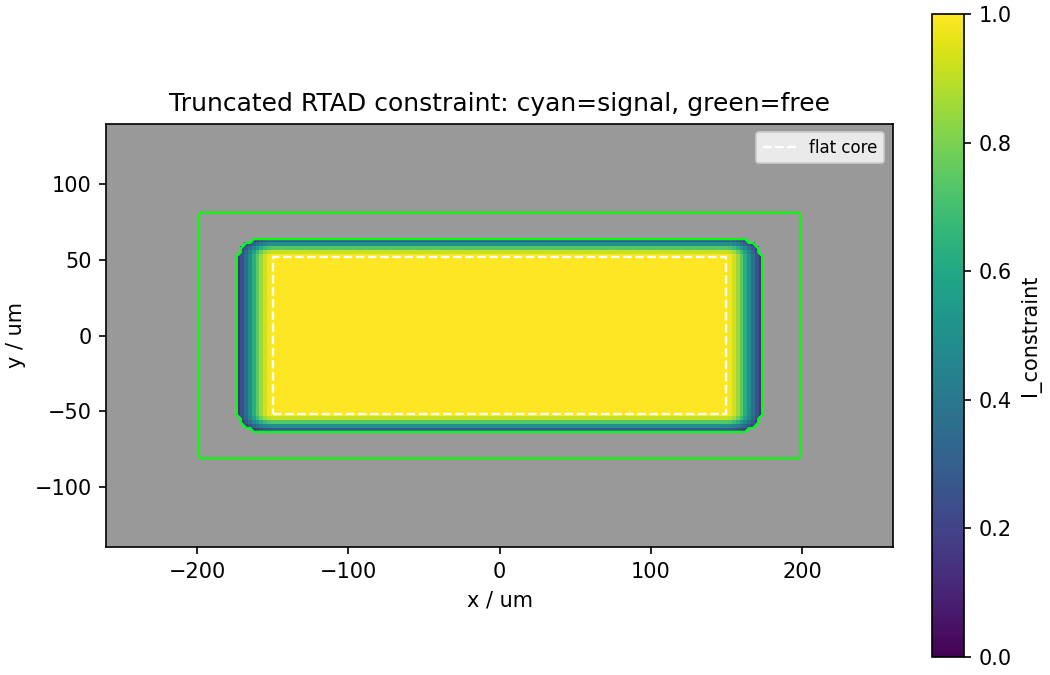
\includegraphics[width=0.72\textwidth]{target_constraint_intensity.png}\\
      {\scriptsize RTAD 约束目标}
      \vspace{0.0cm}
      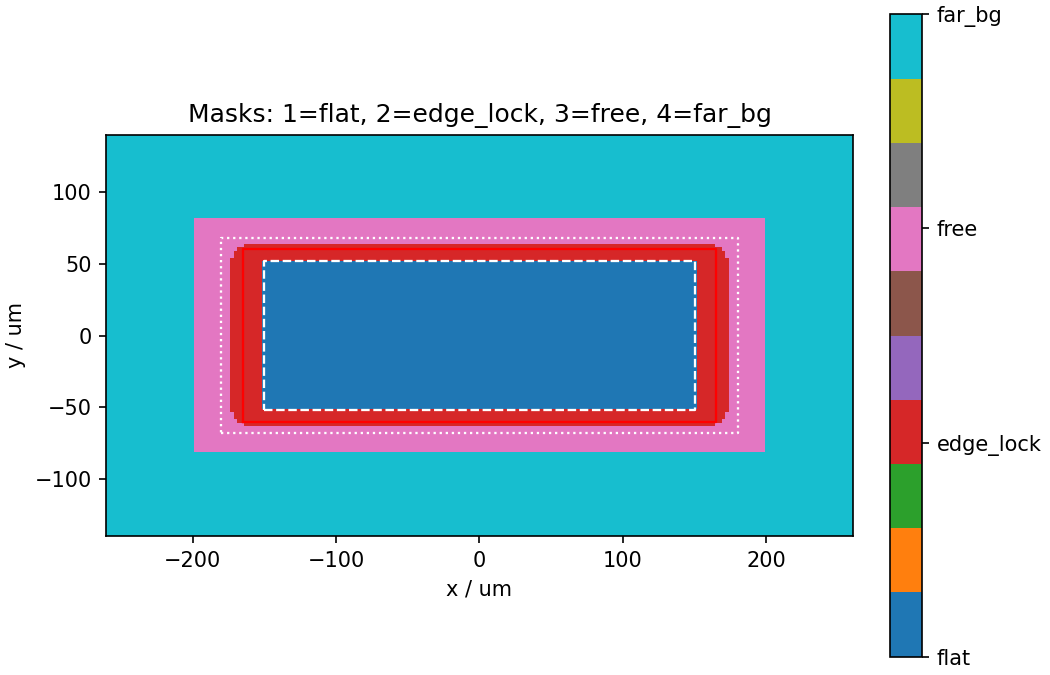
\includegraphics[width=0.72\textwidth]{masks.png}\\
      {\scriptsize 区域划分 (masks)}
    \end{center}
  \end{columns}
\end{frame}

% ===================================================================
\begin{frame}{物理基础 \ \ WGS 优化算法}
  {\footnotesize Alsaka et al., \textit{Applied Physics B}, 128, 137 (2022) \quad$|$\quad 算法参考: slmsuite v0.4.1}

  \vspace{0.1cm}
  \begin{enumerate}
    \item 前向 FFT：DOE 面 $\to$ 焦面复振幅
    \item \textbf{MRAF 投影}：$E'_{\mathrm{signal}} = A_{\mathrm{target}} e^{i\arg(E)}$,\;
      $E'_{\mathrm{free}} = m E$,\; $E'_{\mathrm{bg}} = b E$
    \item 逆向 FFT 回 DOE 面，提取新相位
    \item \textbf{WGS 权重反馈} (仅 mask\_flat 内):
  \end{enumerate}
  \[
    w \leftarrow w\cdot\bigl(\tfrac{\langle|E_{\mathrm{flat}}|\rangle}{|E|}\bigr)^{\gamma},\;
    w = \mathrm{clip}(w,\,0.5,\,2.0),\;
    w\; /\!= \langle w\rangle
  \]
\end{frame}

% ===================================================================
\begin{frame}{物理基础 \ \ WGS 优化结果}
  \begin{columns}
    \column{0.5\textwidth}
    \begin{center}
      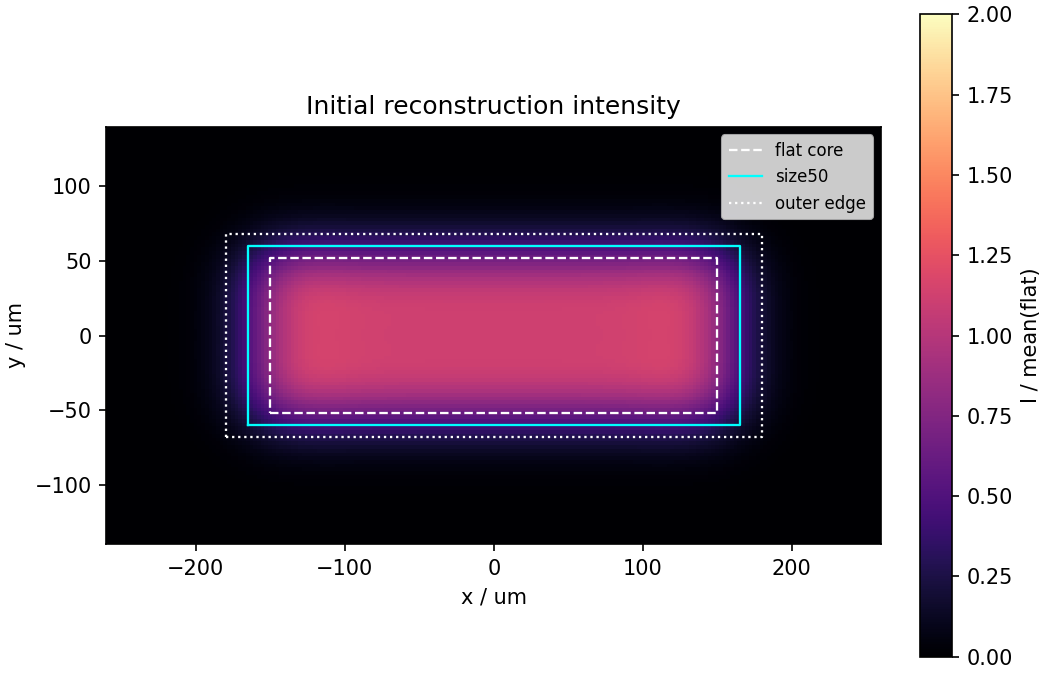
\includegraphics[width=0.92\textwidth]{initial_reconstruction_intensity.png}\\
      {\footnotesize 优化前 (Phase0) \quad RMS $\gg$ 1.86\%}
    \end{center}
    \column{0.5\textwidth}
    \begin{center}
      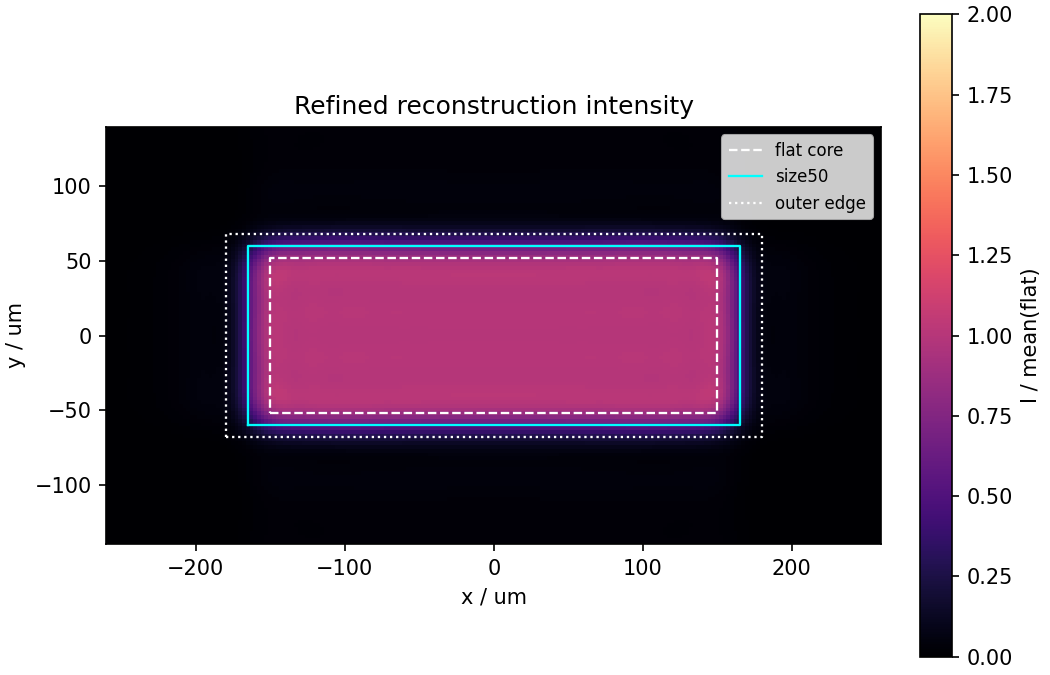
\includegraphics[width=0.92\textwidth]{refined_reconstruction_intensity.png}\\
      {\footnotesize 优化后 (WGS 200 iter) \quad RMS = 1.86\%}
    \end{center}
  \end{columns}

  \vspace{0.05cm}
  \begin{center}
    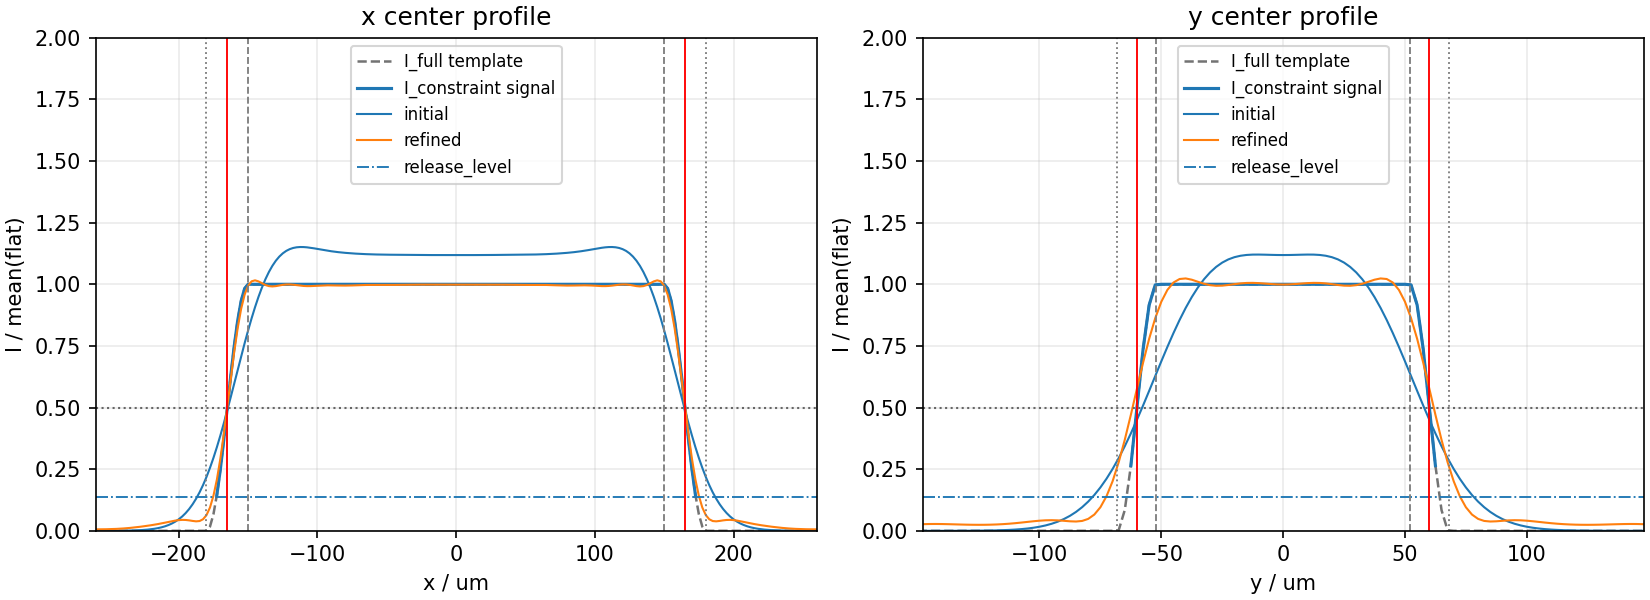
\includegraphics[width=0.62\textwidth]{center_profiles_compare.png}\\
    {\footnotesize 优化前后中心剖面对比 (x/y) —— 平台均匀性显著改善}
  \end{center}
\end{frame}

% ===================================================================
\begin{frame}{物理基础 \ \ 优化策略要点}
  \begin{columns}
    \column{0.55\textwidth}
    \textbf{核心经验}:
    \begin{itemize}
      \item[\orange{$\star$}] \textbf{不约束远背景} ($b_{\mathrm{bg}}\!\to\!1.0$) 是最大单项改进
      \item[\orange{$\star$}] 直接 WGS 优于 MRAF-only 和 MRAF$\to$WGS 混合
    \end{itemize}

    \textbf{工作参数}:
    \footnotesize
    \begin{itemize}
      \item method = wgs\quad strategy = flat\_local
      \item iterations = 200\quad feedback\_exponent = 0.8
      \item weight range = [0.5, 2.0]
      \item mraf\_factor = 0.8\quad bg\_factor = 1.0
    \end{itemize}

    \column{0.45\textwidth}
    \begin{center}
      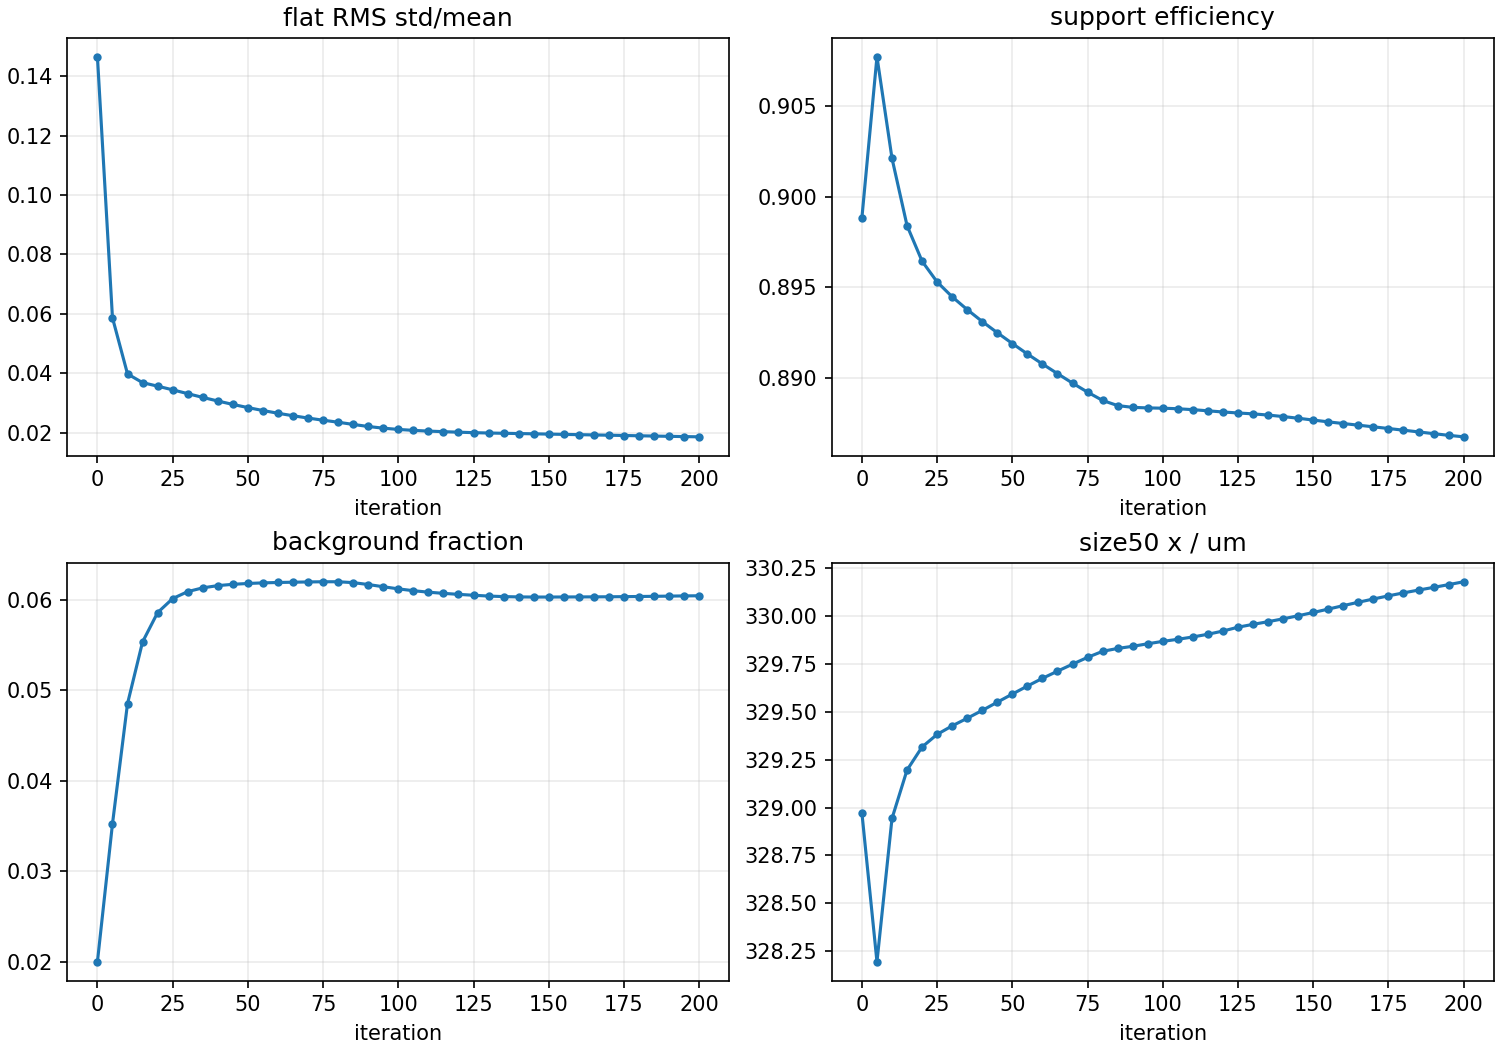
\includegraphics[width=0.90\textwidth]{convergence_metrics.png}\\
      {\footnotesize 收敛曲线}
    \end{center}
  \end{columns}

  \begin{center}
    \scriptsize
    \orange{\textbf{基线结果:~~size50 = $330.2\!\times\!123.6\,\mu$m~~$|$~~RMS = 1.86\%~~$|$~~$e^{-2}$ 效率 = 92.5\%}}
  \end{center}
\end{frame}

% ===================================================================
\section{容差评估}

\begin{frame}{真实光路容差评估}
  \textbf{目标}: 固定设计好的 DOE 相位，仅改变光路/入射条件，评估 DOE 鲁棒性

  \vspace{0.1cm}
  \begin{table}
    \rowcolors{2}{gray!10}{white}
    \small
    \begin{tabular}{lll}
      \toprule
      \textbf{误差类型} & \textbf{参数} & \textbf{物理含义} \\
      \midrule
      离焦 & defocus\_mm & 观察面偏离焦平面 $\pm 2$mm \\
      光束偏移 & offset\_x/y\_mm & 光斑偏离 DOE 中心 $\pm 0.5$mm \\
      光束尺寸 & diameter\_1e2\_mm & 入射光斑尺寸 3.5$\sim$6.5mm \\
      发散/会聚 & divergence\_edge\_mrad & DOE 面波前曲率 $\pm 0.5$mrad \\
      倾角 & pointing\_shift\_um & 光束倾斜$\to$焦斑平移 $\pm 100\mu$m \\
      通光孔径 & clear\_aperture\_mm & 有效通光区域 10$\sim$15mm \\
      椭圆度 & Dx / Dy & x/y 光斑尺寸不一致 \\
      \bottomrule
    \end{tabular}
  \end{table}

  \begin{center}
    \tiny 每种误差独立扫描 + 双参数组合扫描定位耦合效应
  \end{center}
\end{frame}

% ===================================================================
\begin{frame}{问题  --  长边中间内凹  $\to$  椭圆度 $D_x > D_y$}
  \begin{columns}[T]
    \column{0.33\textwidth}
    \centering
    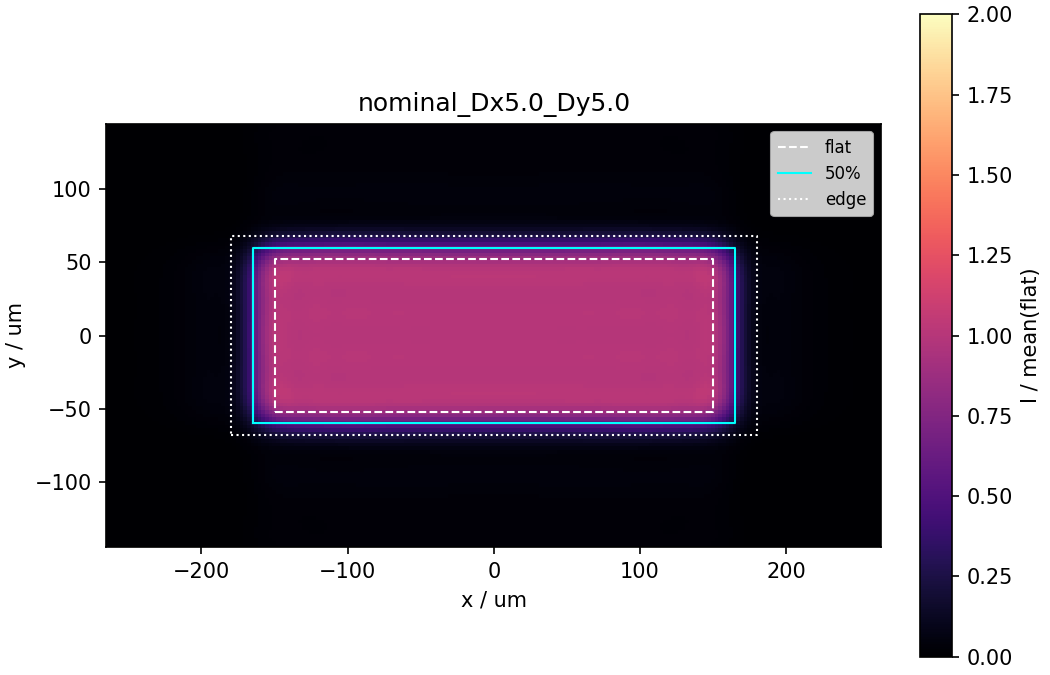
\includegraphics[width=\textwidth]{intensity_nominal_Dx5p0_Dy5p0.png}\\[2pt]
    {\footnotesize nominal: $D_x\!=\!D_y\!=\!5.0$mm}
    \column{0.33\textwidth}
    \centering
    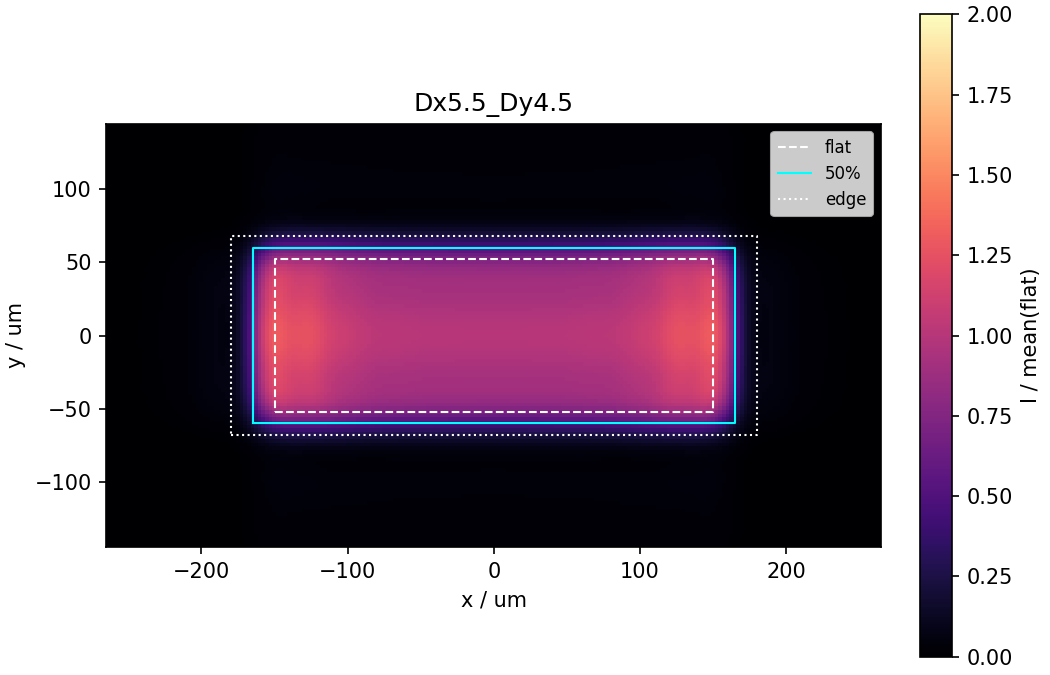
\includegraphics[width=\textwidth]{intensity_Dx5p5_Dy4p5.png}\\[2pt]
    {\footnotesize $D_x\!=\!5.5$,\, $D_y\!=\!4.5$mm \quad 内凹+5.8$\mu$m}
    \column{0.33\textwidth}
    \centering
    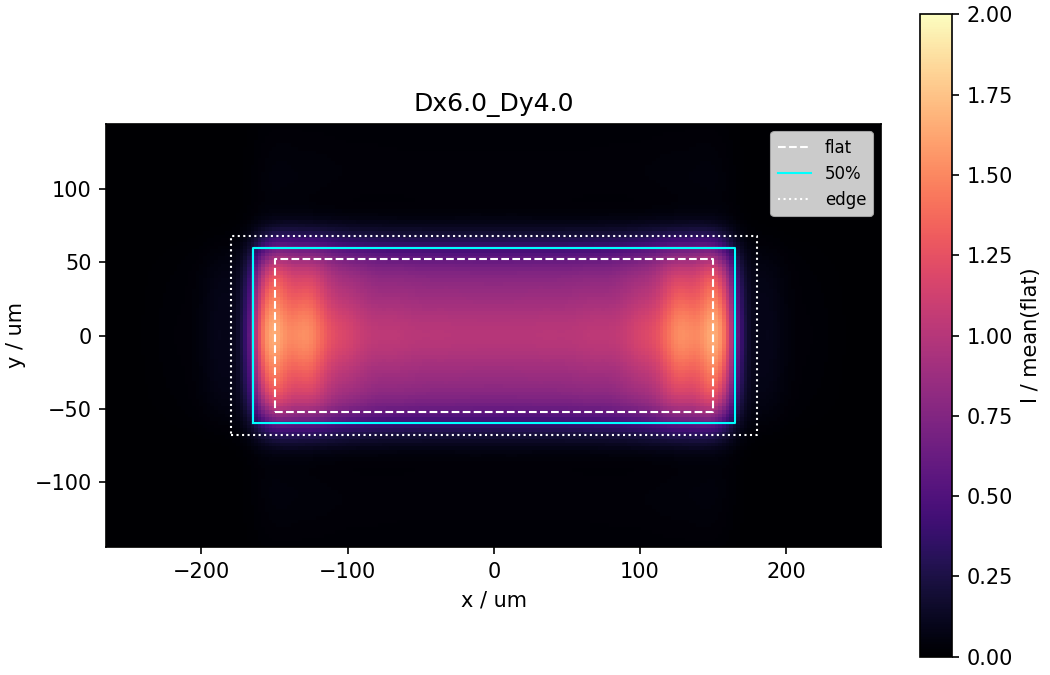
\includegraphics[width=\textwidth]{intensity_Dx6p0_Dy4p0.png}\\[2pt]
    {\footnotesize $D_x\!=\!6.0$,\, $D_y\!=\!4.0$mm \quad 内凹+12.8$\mu$m}
  \end{columns}

  \vspace{0.2cm}
  \begin{itemize}
    \item \orange{机制}: x 方向过度照明，抢走长边中心处 y 向能量 $\to$ 长边 (330$\mu$m 边) 中段内凹
    \item 仅缩小 $D_y$ 而保持 $D_x\!=\!5.0$ 几乎不产生内凹 —— 必须 $D_x > D_y$
  \end{itemize}
\end{frame}

% ===================================================================
\begin{frame}{问题  --  四条边都内凹  $\to$  负离焦 + 光斑偏大}
  \begin{columns}[T]
    \column{0.25\textwidth}
    \centering
    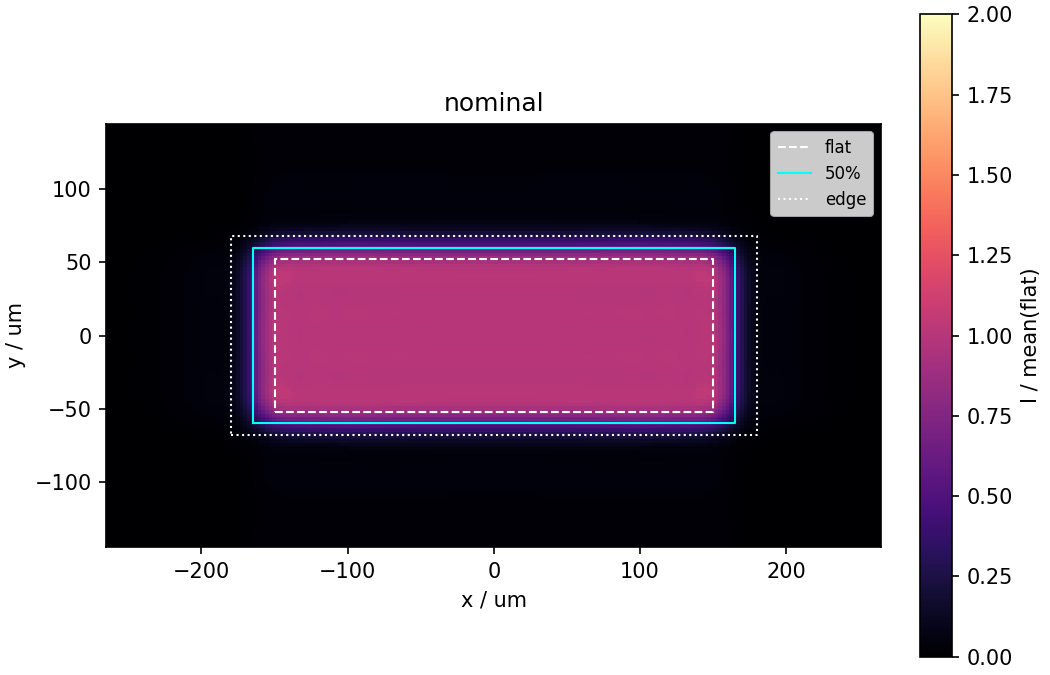
\includegraphics[width=\textwidth]{intensity_nominal_p3.png}\\[2pt]
    {\footnotesize nominal}
    \column{0.25\textwidth}
    \centering
    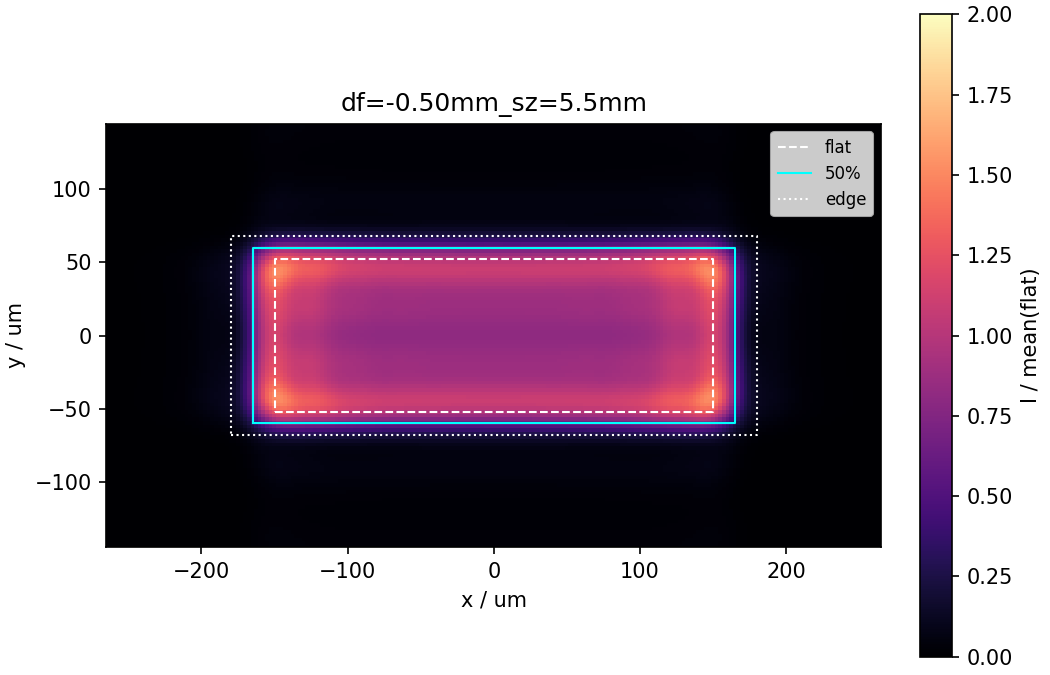
\includegraphics[width=\textwidth]{intensity_df=m0p50mm_sz=5p5mm.png}\\[2pt]
    {\footnotesize $df\!=\!-0.5$, $sz\!=\!5.5$mm}
    \column{0.25\textwidth}
    \centering
    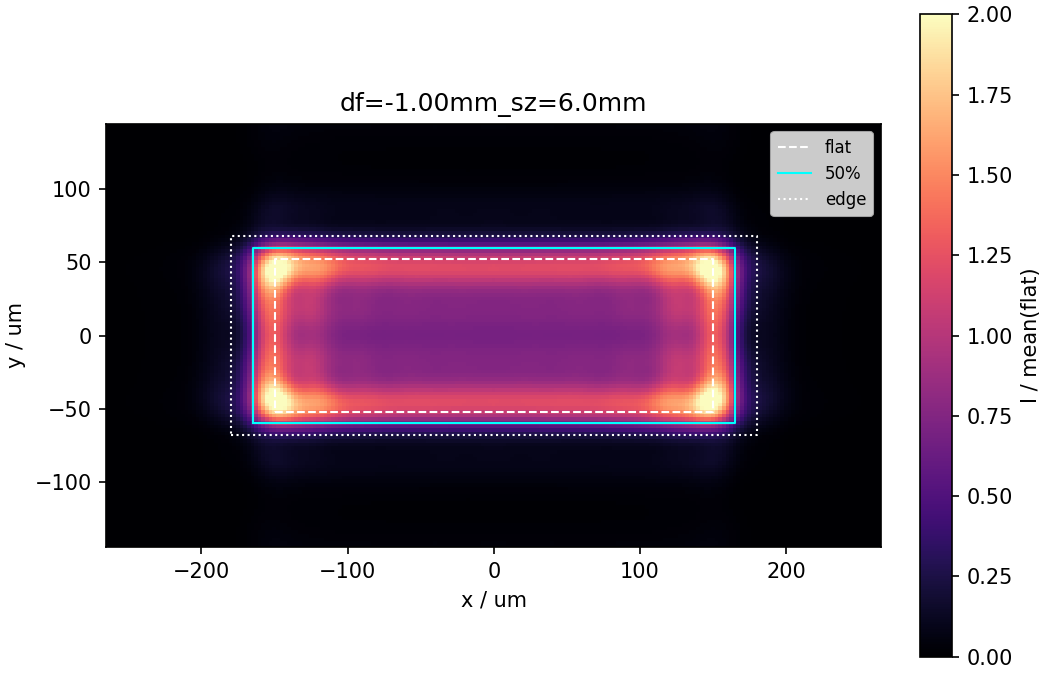
\includegraphics[width=\textwidth]{intensity_df=m1p00mm_sz=6p0mm.png}\\[2pt]
    {\footnotesize $df\!=\!-1.0$, $sz\!=\!6.0$mm}
    \column{0.25\textwidth}
    \centering
    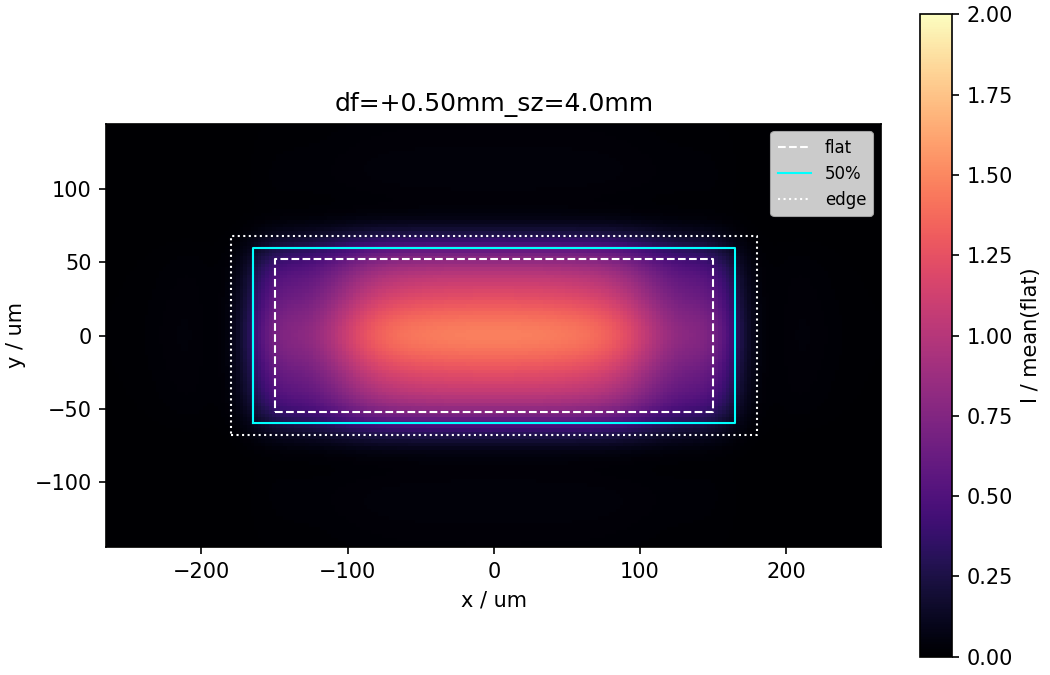
\includegraphics[width=\textwidth]{intensity_df=p0p50mm_sz=4p0mm.png}\\[2pt]
    {\footnotesize 对照: $df\!=\!+0.5$, $sz\!=\!4.0$mm}
  \end{columns}

  \vspace{0.2cm}
  \begin{itemize}
    \item \orange{四边内凹条件}: 负离焦 ($-0.25\sim-1.0$mm) $+$ 光斑偏大 ($\geq 5.5$mm) $\to$ x\_conc 和 y\_conc 同时为正
    \item 小光斑 + 离焦 $\to$ 四边外凸 (右图)；纯离焦无法同时四边内凹
  \end{itemize}
\end{frame}

% ===================================================================
\begin{frame}{问题  --  长边能量缺失 + 短边倾斜  $\to$  beam\_offset}
  \begin{columns}[T]
    \column{0.5\textwidth}
    \centering
    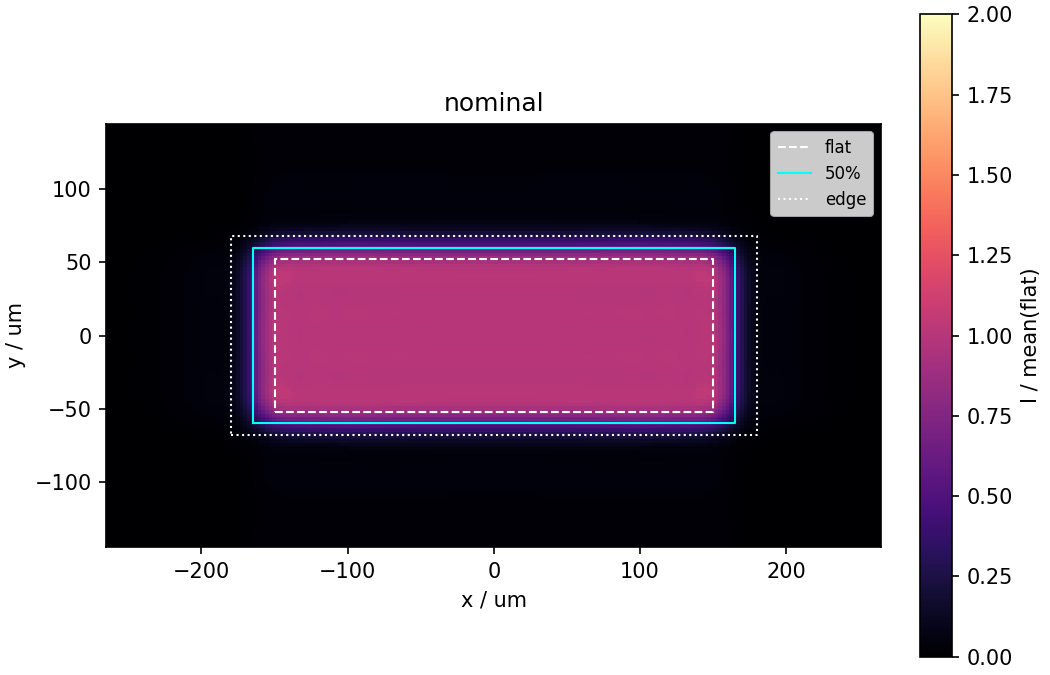
\includegraphics[width=\textwidth]{intensity_nominal_p2.png}\\[2pt]
    {\footnotesize nominal}
    \column{0.5\textwidth}
    \centering
    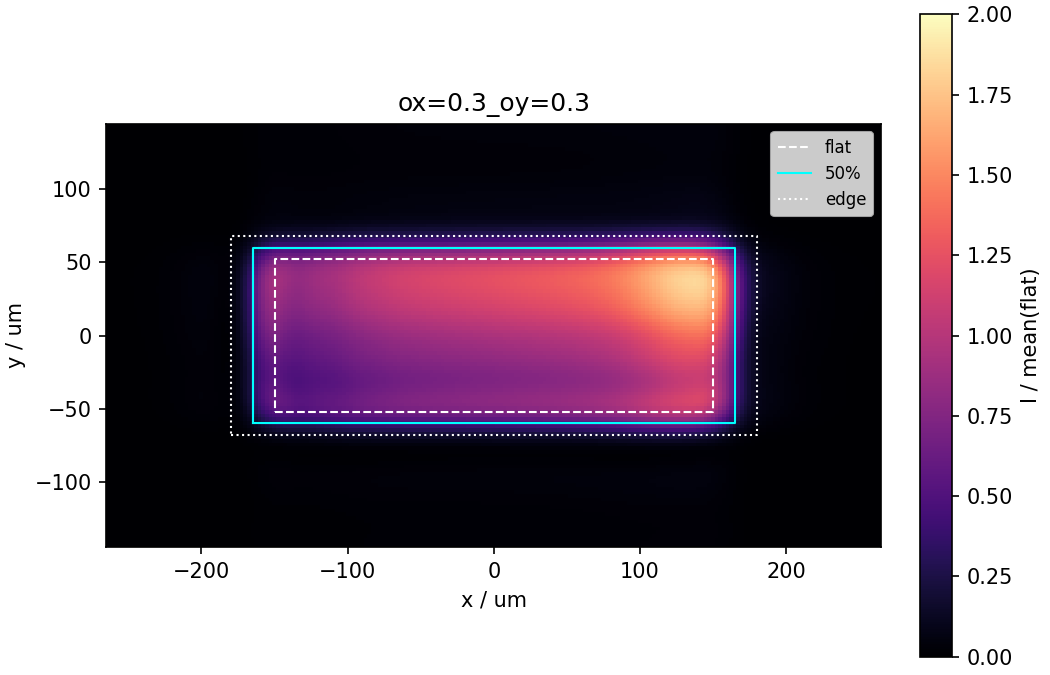
\includegraphics[width=\textwidth]{intensity_ox=0p3_oy=0p3.png}\\[2pt]
    {\footnotesize $offset_x\!=\!0.3$mm, $offset_y\!=\!0.3$mm}
  \end{columns}

  \vspace{0.15cm}
  \begin{itemize}
    \item 光斑偏离 DOE 中心 $\to$ 不对称照明 $\to$ 一侧长边能量缺失
    \item 复合偏移 (x+y) 更接近实际误差形态（排除 H3 offset+pointing 仅偏离 target 的可能）
  \end{itemize}
\end{frame}

% ===================================================================
\begin{frame}{问题  --  能量上下聚集 $\to$  beam\_size}
  \begin{center}
    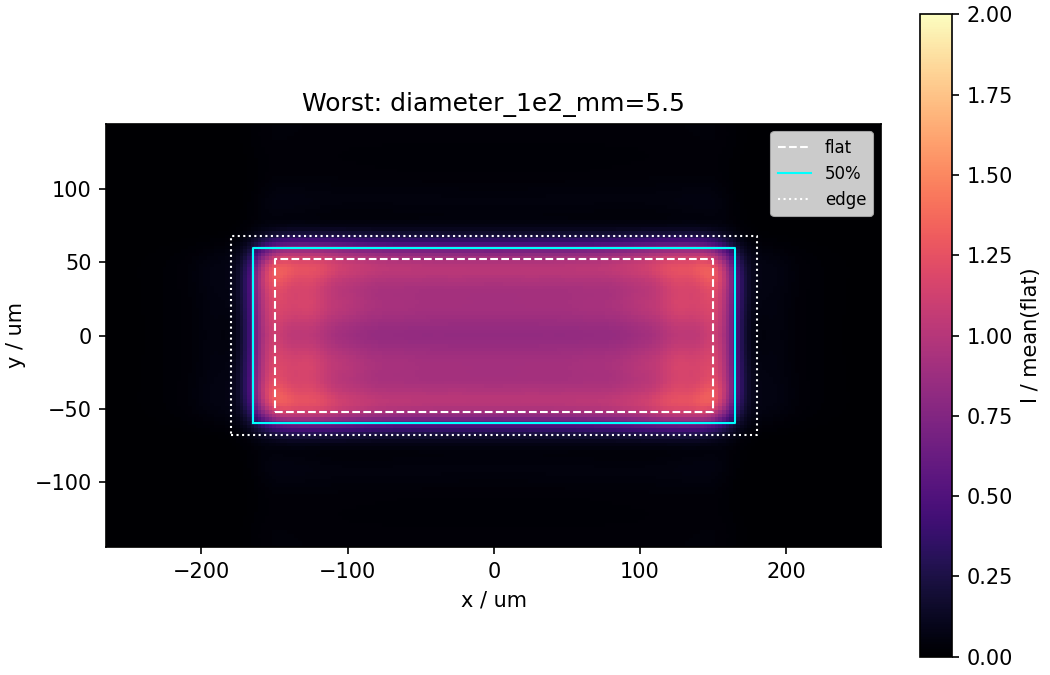
\includegraphics[width=0.65\textwidth]{BEAMSIZE/representative_intensity_worst.png}\\
  \end{center}
  \vspace{0.15cm}
  \begin{itemize}
    \item 入射光斑尺寸 ($1/e^2$ 直径) 偏离名义值 5mm $\to$ 改变 y 向照明轮廓
    \item 光斑偏大 $\to$ 上下边缘能量聚集；光斑偏小 $\to$ 外围欠照明
  \end{itemize}
\end{frame}

% ===================================================================
\section{项目架构}

\begin{frame}[fragile]{项目架构}
  \scriptsize
  \begin{verbatim}
Point2P/
├── initial_phase_generation/   [MATLAB]  Romero-Dickey 初始相位
│   └── generate_initial_phase.m   核心: 稳相法解析相位
├── rtad_mraf_gs_python/        [Python]  MRAF/WGS 迭代优化
│   ├── src/mraf_gs.py             核心: GS/MRAF/WGS 精化循环
│   ├── src/rtad_target.py         RTAD 升余弦矩形目标构建
│   └── run_rtad_mraf_gs_case.py   CLI 入口
├── real_world_simulation/      [Python]  真实光路容差评估
│   ├── src/field_models.py        真实入射场 (偏移/发散/倾角)
│   ├── src/propagation.py         传播 + 角谱法离焦
│   └── run_real_world_sweep.py    CLI 扫描入口
├── result_diagnostics/         [MATLAB]  焦平面诊断 (备用)
└── text/                       参考文献 (x4)
  \end{verbatim}
\end{frame}

% ===================================================================
\begin{frame}{项目架构 \ \ 实验光路}
  \begin{center}
    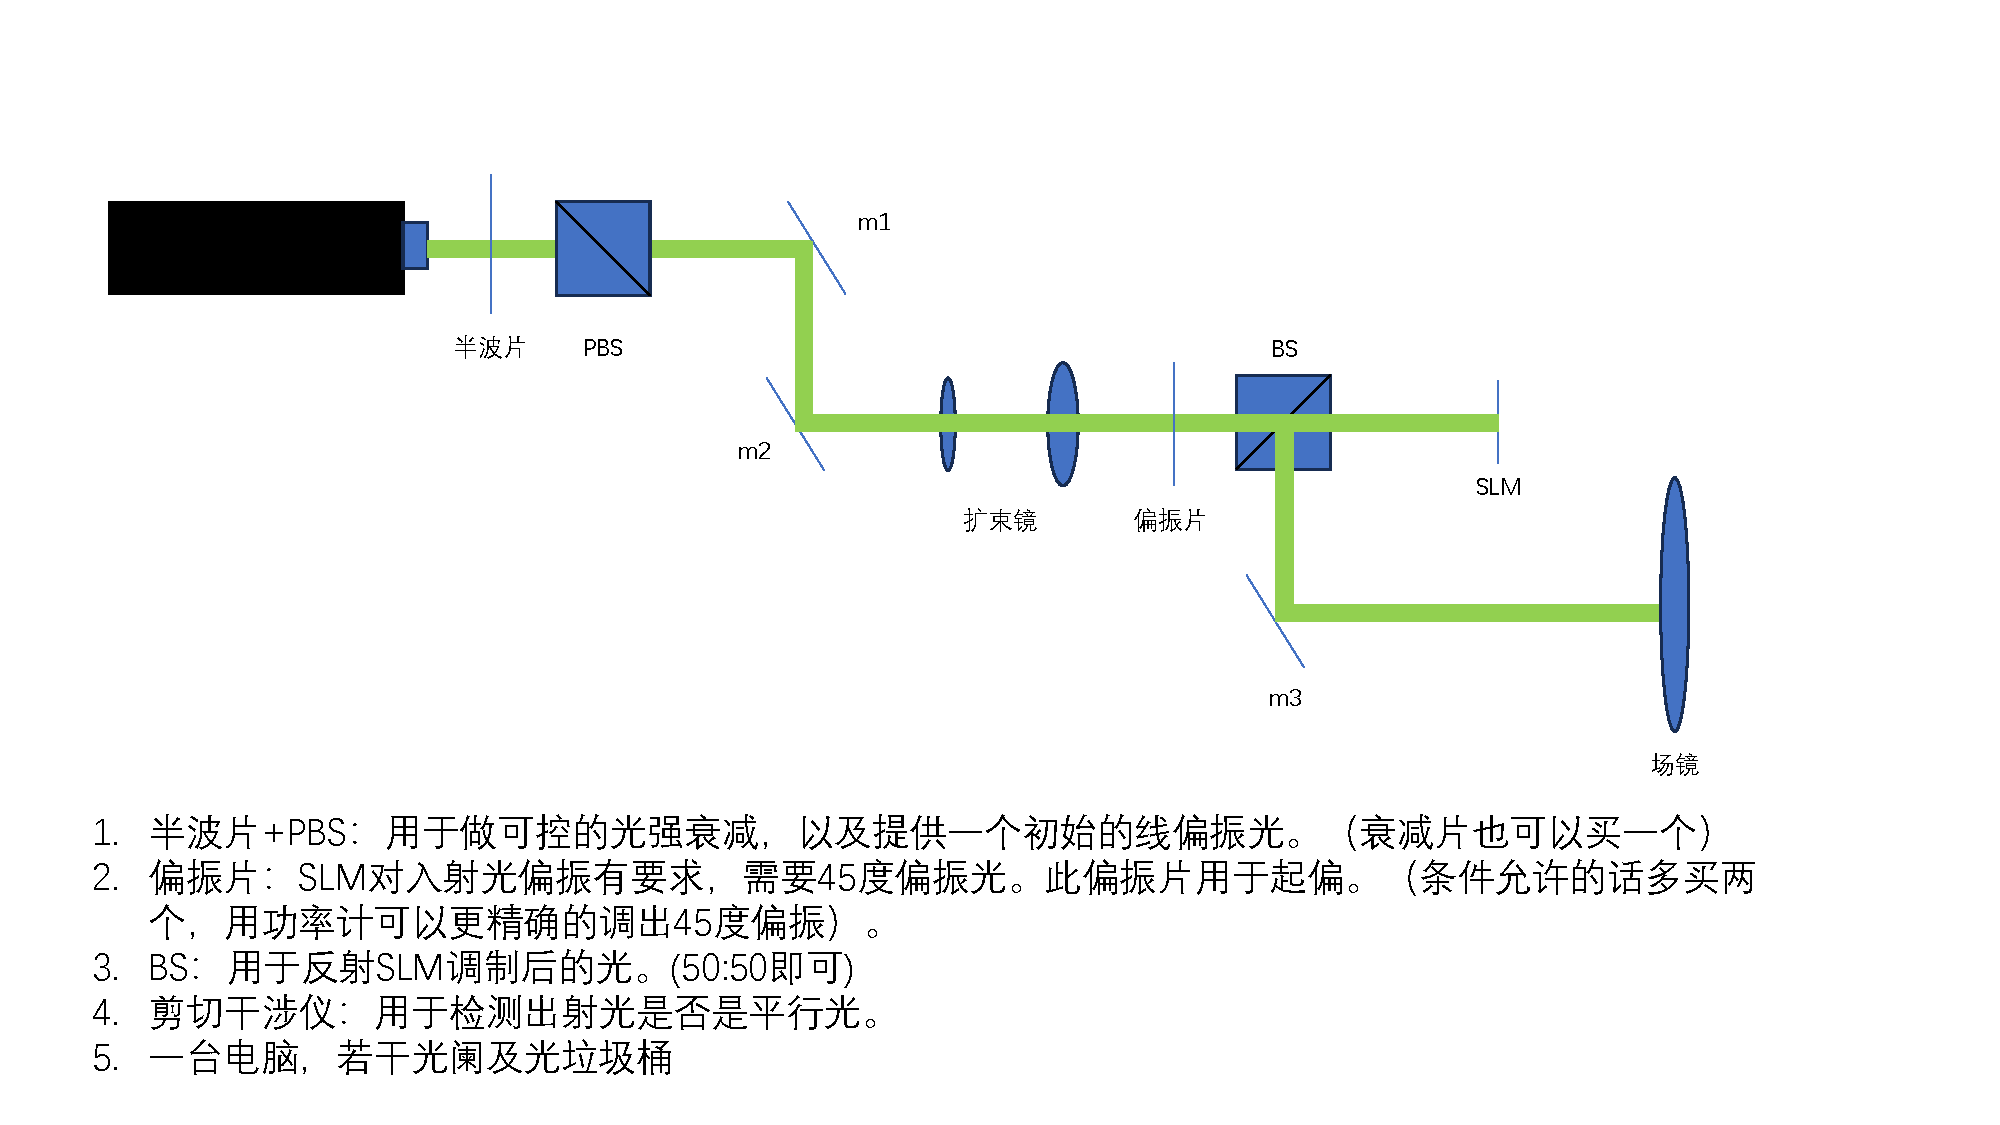
\includegraphics[width=0.85\textwidth]{光路图.pdf}\\
    \vspace{0.15cm}
    {\footnotesize DOE 面（输入高斯）$\;\to\;$ 傅里叶透镜（$f=429$\,mm）$\;\to\;$ 焦平面观测}
  \end{center}
\end{frame}

% ===================================================================
\section{总结}

\begin{frame}{总结}
  \begin{enumerate}
    \item \textbf{Point2P 初始相位}
    \begin{itemize}
      \item Romero-Dickey 解析解 ($\beta_x=9.06$, $\beta_y=3.30$)，物理初值接近目标
    \end{itemize}

    \item \textbf{RTAD 目标函数}
    \begin{itemize}
      \item 升余弦下降边缘抑制频谱泄露；截断约束保留物理旁瓣
    \end{itemize}

    \item \textbf{WGS 优化}
    \begin{itemize}
      \item 直接 flat-local WGS，\orange{不约束远背景} 是最大改进
    \end{itemize}

    \item \textbf{最终结果}
    \begin{itemize}
      \item RMS 非均匀性 = \orange{1.86\%},~~$e^{-2}$ 衍射效率 = \orange{92.5\%}
    \end{itemize}

    \item \textbf{容差分析}
    \begin{itemize}
      \item 揭示 5 类光斑误差的根因 $\to$ 实验反向纠错
    \end{itemize}
  \end{enumerate}

  \vspace{0.05cm}
  \begin{center}
    \footnotesize
    \orange{关键容差量级:~~发散角 $\sim\pm 0.005$\,mrad~~$|$~~离焦 $\sim\pm 0.75$\,mm~~$|$~~偏移 $\sim\pm 0.2$\,mm}
  \end{center}
\end{frame}

% ===================================================================
\begin{frame}{参考文献}
  \begin{enumerate}
    \item Romero, L.A. \& Dickey, F.M. ``Lossless laser beam shaping.''
          \textit{J. Opt. Soc. Am. A}, 13(4), 751--760 (1996).

    \item Chen, W. et al. ``Generation of high uniformity flat-top beams by
          reconstructing the amplitude distribution at descending edges.''
          \textit{Optics \& Laser Technology}, 186, 112776 (2025).

    \item Alsaka, D.Y. et al. ``Dynamic flat-topped laser beam shaping method
          using mixed region amplitude freedom algorithm.''
          \textit{Applied Physics B}, 128, 137 (2022).

    \item Zhang, C. et al. ``Optimized holographic femtosecond laser patterning.''
          \textit{Scientific Reports}, 6, 33281 (2016).

    \item slmsuite v0.4.1 --- github.com/slmsuite/slmsuite
  \end{enumerate}
\end{frame}

\end{document}
